% SC4242 --- Chapter 2: Lexical Analysis & NFA->DFA (0->100 ground-up)
\chapter{Lexical Analysis: From Regex to DFA}
\label{ch:lexical}

\begin{quote}
\emph{``Scanning is pattern matching made deterministic.''} --- Regular expressions describe tokens; NFAs execute them speculatively; DFAs execute them deterministically at bytes-per-cycle speed.
\end{quote}

\noindent\fbox{\parbox{\dimexpr\linewidth-2\fboxsep-2\fboxrule}{%
\textbf{From zero: we build here, no automata assumed beyond sets.} We define alphabets, languages, and regular expressions from scratch (recapping SC2203 Ch.~2 in one page), then build Thompson NFAs, $\varepsilon$-closure, subset construction, and minimisation. Pictures precede formalism throughout.}}
\vspace{0.4em}

\section*{Learning Outcomes}
After this chapter you will be able to:
\begin{enumerate}[label=(L\arabic*)]
    \item write regular expressions for tokens (keywords, identifiers, numbers, strings);
    \item build a Thompson $\varepsilon$-NFA from a regex and argue its size is linear;
    \item compute $\varepsilon$-closure and simulate an NFA on an input string;
    \item convert NFA$\to$DFA via subset construction and minimise via partition refinement;
    \item implement maximal-munch lexing with priority and emit a token stream with spans.
\end{enumerate}

% ============================================================
\section{Regular Expressions for Tokens}
\label{sec:regex-tokens}
\emph{Intuition:} a token is a \emph{lexeme} matched by a pattern: ``identifier looks like a letter followed by letters/digits''. Regexes name those patterns precisely.

Fix alphabet $\Sigma$ (e.g., ASCII $0$--$127$). A \emph{language} is a set $L\subseteq\Sigma^*$.
\begin{definition}[Regex syntax and $L(\cdot)$]
Basis: $\emptyset$ with $L=\emptyset$, $\varepsilon$ with $L=\{\varepsilon\}$, $a$ ($a\in\Sigma$) with $L=\{a\}$. If $R,S$ are regexes then $(R|S)$ is union ($L(R)\cup L(S)$), $(RS)$ concatenation ($\{xy\mid x\in L(R),y\in L(S)\}$), $(R^*)$ star ($\bigcup_{n\ge0}L(R)^n$). Shorthand: $R^+=RR^*$, $R?=R|\varepsilon$, $[a\text{-}z]$ enumerates, $R\{m,n\}$ bounded repeat, ``.'' is $\Sigma\setminus\{\backslash n\}$.
\end{definition}
Precedence: $*$ highest, concat next, $|$ lowest; so \texttt{ab|cd*} means \texttt{(ab)|(c(d*))}.

\begin{example}[Token patterns]
\texttt{if} keyword: \texttt{if} (exact). Identifier: \texttt{[a-zA-Z\_][a-zA-Z0-9\_]*}. Integer: \texttt{0|[1-9][0-9]*}. Hex: \texttt{0x[0-9a-fA-F]+}. String: \texttt{"[{\string^}"]*"} (ignoring escapes for now). Whitespace/comments are tokens too, just discarded.
\end{example}

A lexer has \emph{many} regexes $R_1,\dots,R_k$ (one per token kind). We combine them as $R = (R_1|R_2|\dots|R_k)$ tagged by kind and priority (keywords beat identifiers when both match \texttt{if}).

% TikZ 1: Thompson fragments
\begin{figure}[h]
\centering
\begin{tikzpicture}[>=Stealth,scale=0.78,every node/.style={font=\scriptsize}]
\tikzstyle{st}=[draw,circle,fill=white,minimum size=5mm,inner sep=0pt]
% fragment a
\begin{scope}
\node[st,fill=blue!12] (a0) at (0,1.6) {};
\node[st,fill=green!14] (a1) at (1.7,1.6) {};
\draw[->,thick,blue!60!black] (a0)--(a1) node[midway,above] {$a$};
\node[font=\tiny] at (0.85,1.05) {symbol $a$};
\end{scope}
% fragment concat
\begin{scope}[xshift=3.0cm]
\node[st,fill=blue!12] (b0) at (0,1.6) {};
\node[st] (b1) at (1.4,1.6) {};
\node[st,fill=green!14] (b2) at (2.8,1.6) {};
\draw[->,thick] (b0)--(b1) node[midway,above,font=\tiny] {$R_1$};
\draw[->,dashed,red!60!black] (b1)--(b2) node[midway,above,font=\tiny] {$\varepsilon$};
\node[font=\tiny] at (1.4,1.05) {$R_1R_2$ (chain)};
\end{scope}
% fragment union
\begin{scope}[xshift=6.4cm]
\node[st,fill=blue!12] (c0) at (0,1.6) {};
\node[st] (c1) at (1.0,2.2) {};
\node[st] (c2) at (1.0,1.0) {};
\node[st,fill=green!14] (c3) at (2.4,1.6) {};
\draw[->,dashed,red!60!black] (c0)--(c1);
\draw[->,dashed,red!60!black] (c0)--(c2);
\draw[->,thick] (c1)--(c3) node[midway,above,font=\tiny] {$R_1$};
\draw[->,thick] (c2)--(c3) node[midway,below,font=\tiny] {$R_2$};
\node[font=\tiny] at (1.2,0.5) {$R_1|R_2$ ($\varepsilon$-fork/join)};
\end{scope}
% fragment star
\begin{scope}[xshift=1.8cm,yshift=-1.55cm]
\node[st,fill=blue!12] (d0) at (0,1.6) {};
\node[st] (d1) at (1.5,1.6) {};
\node[st,fill=green!14] (d2) at (3.0,1.6) {};
\draw[->,dashed,red!60!black] (d0)--(d1);
\draw[->,thick] (d1)--(d2) node[midway,above,font=\tiny] {$R$};
\draw[->,dashed,red!60!black,bend left=28] (d1) to (d0);
\draw[->,dashed,red!60!black,bend right=28] (d2) to (d0);
\draw[->,dashed,red!60!black] (d0) to[bend left=18] (d2);
\node[font=\tiny] at (1.5,0.85) {$R^*$ ($\varepsilon$-loop)};
\end{scope}
\begin{scope}[xshift=6.4cm,yshift=-1.55cm]
\draw[thick,fill=yellow!12,rounded corners=2pt] (0,0.95) rectangle (2.7,2.05);
\node[font=\tiny,align=left] at (1.35,1.5) {legend: \tikz\draw[thick,blue!60!black,->] (0,0)--(0.5,0); solid = consume\\ \tikz\draw[dashed,red!60!black,->] (0,0)--(0.5,0); dashed = $\varepsilon$};
\end{scope}
\end{tikzpicture}
\caption{Thompson fragments: each regex maps to an $\varepsilon$-NFA with one entry and one exit, built inductively in $O(|R|)$ states/edges.}
\label{fig:thompson}
\end{figure}

% ============================================================
\section{From Regex to $\varepsilon$-NFA}
\label{sec:thompson}
\emph{Intuition:} an NFA may be in many states at once---``guess'' which $R_i$ matches. That nondeterminism is exactly what regex union and star mean.

\begin{definition}[Thompson NFA]
For each regex node build fragment above with fresh entry/exit. $\varepsilon$-edges are unlabeled. Sizes add linearly: $|\text{NFA}(R)|\le 2|R|$ states. See Fig.~\ref{fig:thompson}.
\end{definition}
\begin{example}[NFA for \texttt{[a-b]*abb}]
Thompson gives $2$ states per literal plus forks for star and union. The full NFA has $\approx14$ states before trimming; it has parallel $a/b$ branches inside the star. Any regex of length $n$ yields $O(n)$-size NFA in linear time.
\end{example}

% Listing 1: Thompson sketch
\begin{lstlisting}[language=Python]
# Thompson: AST node -> (entry, exit, edges)
def thompson(node, new_state):
    if node.kind == 'lit':          # 'a'
        s, t = new_state(), new_state()
        return (s, t, [(s, node.char, t)])
    if node.kind == 'concat':
        l = thompson(node.left, new_state); r = thompson(node.right, new_state)
        return (l.entry, r.exit, l.edges + r.edges + [(l.exit, None, r.entry)])
    if node.kind == 'alt':          # R|S : epsilon fork/join (Fig.1)
        s, t = new_state(), new_state()
        l = thompson(node.left, new_state); r = thompson(node.right, new_state)
        eps = [(s,None,l.entry),(s,None,r.entry),(l.exit,None,t),(r.exit,None,t)]
        return (s, t, l.edges + r.edges + eps)
    if node.kind == 'star':
        s, t = new_state(), new_state()
        c = thompson(node.child, new_state)
        eps = [(s,None,c.entry),(s,None,t),(c.exit,None,c.entry),(c.exit,None,t)]
        return (s, t, c.edges + eps)
\end{lstlisting}

% ============================================================
\section{Subset Construction: NFA $\to$ DFA}
\label{sec:subset}
To run fast, we remove guessing.

\begin{definition}[$\varepsilon$-closure and move]
$\text{Eclose}(S)$ = all states reachable from $S$ via $\varepsilon^*$. $\text{move}(S,a)=\{t\mid\exists s\in S: s\xrightarrow{a}t\}$. DFA state = subset of NFA states: $Q_D=\mathcal{P}(Q_N)$ (only reachable subsets built lazily).
\end{definition}
Transition: $\delta_D(S,a)=\text{Eclose}(\text{move}(S,a))$. Start $q_{0D}=\text{Eclose}(\{q_{0N}\})$. Accepting if $S\cap F_N\neq\emptyset$ (priority = smallest $R_i$ whose accept in $S$).

\begin{example}[Ends-with-\texttt{01}: NFA $4$ states $\to$ DFA $4$ reachable of $16$]
NFA $q_0\xrightarrow{0,1}q_0$, $q_0\xrightarrow{0}q_1\xrightarrow{1}q_2$ accept. Subset walk: $\{q_0\}\xrightarrow{1}\{q_0\}$, $\xrightarrow{0}\{q_0,q_1\}\xrightarrow{1}\{q_0,q_2\}$ accept, etc. Fig.~\ref{fig:subset} shows lattice climb.
\end{example}

% TikZ 2: subset lattice + moves
\begin{figure}[h]
\centering
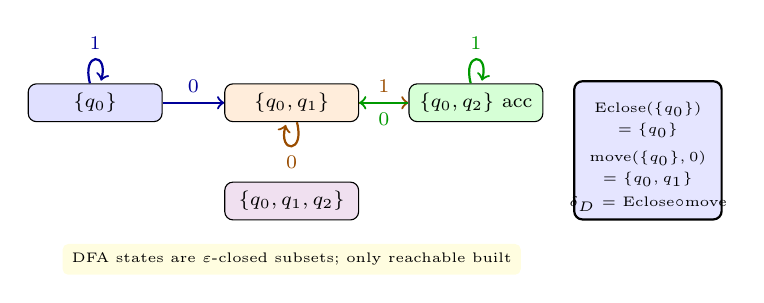
\begin{tikzpicture}[scale=0.78,every node/.style={font=\scriptsize}]
\node[draw,fill=blue!12,rounded corners=3pt,minimum width=1.7cm] (s0) at (0,2.0) {$\{q_0\}$};
\node[draw,fill=orange!14,rounded corners=3pt,minimum width=1.7cm] (s1) at (3.2,2.0) {$\{q_0,q_1\}$};
\node[draw,fill=green!16,rounded corners=3pt,minimum width=1.7cm] (s2) at (6.2,2.0) {$\{q_0,q_2\}$ acc};
\node[draw,fill=violet!12,rounded corners=3pt,minimum width=1.7cm] (s3) at (3.2,0.4) {$\{q_0,q_1,q_2\}$};
\draw[->,thick,blue!60!black] (s0) -- (s1) node[midway,above] {$0$};
\draw[->,thick,blue!60!black] (s0) edge[loop above] node {$1$} (s0);
\draw[->,thick,orange!60!black] (s1) -- (s2) node[midway,above] {$1$};
\draw[->,thick,orange!60!black] (s1) edge[loop below] node {$0$} (s1);
\draw[->,thick,green!60!black] (s2) -- (s1) node[midway,below,sloped] {$0$};
\draw[->,thick,green!60!black] (s2) edge[loop above] node {$1$} (s2);
\node[font=\tiny,fill=yellow!12,rounded corners=2pt] at (3.2,-0.55) {DFA states are $\varepsilon$-closed subsets; only reachable built};
\draw[thick,fill=blue!10,rounded corners=3pt] (7.8,0.1) rectangle (10.2,2.35);
\node[font=\tiny,align=left] at (9.0,1.9) {Eclose$(\{q_0\})$};
\node[font=\tiny] at (9.0,1.55) {$=\{q_0\}$};
\node[font=\tiny,align=left] at (9.0,1.1) {move$(\{q_0\},0)$};
\node[font=\tiny] at (9.0,0.75) {$=\{q_0,q_1\}$};
\node[font=\tiny,align=left] at (9.0,0.35) {$\delta_D$ = Eclose$\circ$move};
\end{tikzpicture}
\caption{Subset construction for \texttt{.*01}: DFA subsets, transitions $\delta_D(S,a)$, and $\varepsilon$-closure (here trivial; with $\varepsilon$ it expands subsets). Hopcroft then merges equivalent DFA states.}
\label{fig:subset}
\end{figure}

\paragraph{Minimisation (Hopcroft).} Start partition $\{F, Q\setminus F\}$; repeatedly split blocks where $a$-successors land in different blocks. Runs $O(|Q|\log|Q|)$ and yields the unique minimal DFA. Lexer tables shrink dramatically.

% ============================================================
\section{Lexing: Maximal Munch, Priority, Spans}
\label{sec:lexing}
With DFA in hand, lexing is a loop: from current input position $p$, run DFA feeding characters until stuck; last accept position gives longest prefix (maximal munch). If tie (e.g., \texttt{if} matches both keyword and identifier regex), choose smallest-index regex (priority). Emit token with span $[p, q)$, advance to $q$, skip whitespace/comments or emit them for tooling. On no accept, emit error at $p$ and resynchronise (e.g., skip to next whitespace).

\begin{example}[Lexing \texttt{if (x<=10)}]
DFA run: \texttt{if}$\to$ keyword \texttt{IF} (priority over \texttt{ID}), \texttt{(}$\to$ \texttt{LPAREN}, \texttt{x}$\to$ \texttt{ID}, \texttt{<=}$\to$ \texttt{LE} (longest: \texttt{<} alone is \texttt{LT} but \texttt{<=} longer), \texttt{10}$\to$ \texttt{INT}. Token stream fed to parser; whitespace dropped but line:col kept.
\end{example}

% Listing 2: lex loop with priority
\begin{lstlisting}[language=Python]
def lex(dfa, text, kinds):
    pos, n, out = 0, len(text), []
    while pos < n:
        state, last_accept, last_pos = dfa.start, None, pos
        i = pos
        while i < n and (state := dfa.delta.get((state, text[i]))) is not None:
            i += 1
            if state in dfa.accept:           # remember last accept
                last_accept, last_pos = state, i
        if last_accept is None:               # no token
            raise LexError(f"illegal char {text[pos]!r} at {pos}")
        kind = kinds[last_accept]             # priority already in accept tag
        lexeme = text[pos:last_pos]
        if kind not in ('WS','COMMENT'):
            out.append((kind, lexeme, pos, last_pos))
        pos = last_pos                        # maximal munch advance
    return out
\end{lstlisting}

% TikZ 3: maximal munch vs priority diagram
\begin{figure}[h]
\centering
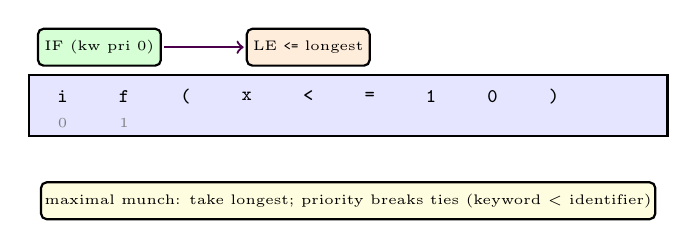
\begin{tikzpicture}[scale=0.78,every node/.style={font=\scriptsize}]
\draw[thick,fill=blue!10] (0,0) rectangle (10.4,1.0);
\foreach \i/\ch in {0/i,1/f,2/(,3/x,4/<,5/=,6/1,7/0,8/)} {\node at (0.55+\i*1.0,0.65) {\texttt{\ch}};}
\node[font=\tiny,gray] at (0.55,0.22) {0};
\node[font=\tiny,gray] at (1.55,0.22) {1};
\draw[thick,fill=green!16,rounded corners=2pt] (0.15,1.15) rectangle (2.15,1.75);
\node[font=\tiny] at (1.15,1.45) {IF (kw pri 0)};
\draw[thick,fill=orange!14,rounded corners=2pt] (3.55,1.15) rectangle (5.55,1.75);
\node[font=\tiny] at (4.55,1.45) {LE \texttt{<=} longest};
\draw[->,thick,violet!60!black] (2.2,1.45)--(3.5,1.45);
\draw[thick,fill=yellow!12,rounded corners=2pt] (0.2,-0.75) rectangle (10.2,-1.35);
\node[font=\tiny] at (5.2,-1.05) {maximal munch: take longest; priority breaks ties (keyword $<$ identifier)};
\end{tikzpicture}
\caption{Lexing decisions: longest prefix wins; on equal length, earliest regex (keywords) wins. Spans $[l,r)$ kept per token for diagnostics and incremental re-lexing.}
\label{fig:munch}
\end{figure}

% ============================================================
\section{Chapter Notes}
Thompson (1968) introduced regex$\to$NFA for QED editor; subset construction is Rabin--Scott (1959); Hopcroft (1971) $O(n\log n)$ minimisation is optimal. Flex and RE2 still use Thompson + DFA with on-demand subset. Unicode, UTF-8 decoding, and longest-match with look-ahead (\texttt{/} trailing context) extend the core; RE2 and Rust's regex crate document production concerns.

% ============================================================
\section{Exercises}
\label{sec:ch02-exercises}
\begin{enumerate}[label=E2.\arabic*, leftmargin=*, itemsep=0.8em]
\item \textbf{Regex to $\varepsilon$-NFA.} Build Thompson NFA for $(a|b)^*abb$; count states/$\varepsilon$-edges. Show $\varepsilon$-closure of start and trace \texttt{ababb}.
\item \textbf{Subset by hand.} Given NFA $q_0\xrightarrow{\varepsilon}q_1$, $q_0\xrightarrow{a}q_0$, $q_1\xrightarrow{b}q_2$ accept, compute reachable DFA subsets, table $\delta_D$, and minimise. Which 2 states merge?
\item \textbf{Maximal munch counterexample.} Regexes: \texttt{IF} \texttt{if} pri 0, \texttt{ID} \texttt{[a-z]+} pri 1, \texttt{WS} \texttt{[ ]+} pri 2. Lex \texttt{iff iffy if}. List tokens and state where priority vs.\ length matters.
\item \textbf{Keyword vs.\ identifier DFA.} Construct combined NFA for \{\texttt{if},\texttt{int},\texttt{[a-zA-Z\_]\textbackslash w*}\} with tagged accepts, subset-construct, show why \texttt{if} is not \texttt{ID} (tag = smallest index). What NFA/DFA size?
\item \textbf{Error recovery.} Input \texttt{"unterminated} (no closing quote) stalls DFA with no accept. Design two policies: (a) error token to next quote, (b) single-token resync to next whitespace; trade-offs for diagnostics and parser recovery.
\end{enumerate}
% End of Chapter 2
